% !TeX spellcheck = en_US
those tips are collected from \href{https://www.carbon111.com/mwxt.html}{Carbon111}
\subsection{An Extra LFO from Modifiers}
A cool way to generate a third LFO to use for that extra touch of animation for your monster sound! Submitted by Rizacan.\\
An extra LFO won't disturb anyone! Here's a little LFO idea using Modifiers as below.
\bigskip % Add an empty line
%These are optional parameters to finetune the placement of tables and figures, with the following meaning:
%
%h, here
%t, top
%b, bottom
%p, page of float
%e.g. \begin{figure}[!htb]
\begin{figure}[ht!]
	\centering
	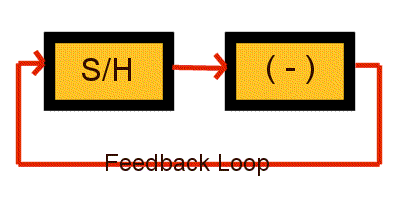
\includegraphics[width=90mm]{pics\lfo_feedback.png}
	\caption{Create a third LFO.}
	\label{third_lfo}
\end{figure}
S/H rate control input sets the overall frequency. Using the filter Modifier, you can get triangle waves. It can also be used for PWM, freeing up other LFOs for other uses!\\
Here are Two examples in Sysex format: \href{https://www.carbon111.com/sysex.zip}{two Examples}
The first one: ``ModifierLFO'' is a simple LFO example. Modifier 1 creates the squarewave and Modifier 3 smoothes the output of Modifier 1 (or 2).\\
The second one, ``Janmichelphaser'', is a simple solina string simulation with a phaser. Modifier 3 produces a triangle waveform using Modifier 1's square wave and modulates PW.
\subsection{Wavetable Browser}
A nice tutorial to create a patch that will allow you to fully audition each of the XT's wavetables. Actually rather handy! Submitted by vanHouten.\\
